\section{Introduction}
The dominant approaches to reinforcement learning rely on a fixed
state-action space and reward function that the agent is trying to
maximize.  During training, the agent is repeatedly reset to a
predefined initial state or set of initial states.  For example, in
the classic RL Mountain Car domain, the agent starts at some point in
the valley, continues until it reaches the top of the valley and then
resets to somewhere else in the same valley. Learning in this regime
is akin to the learning problem faced by Bill Murray in the 1993 movie
{\em Groundhog Day} in which he repeatedly relives the same day, until
he discovers the optimal policy and escapes to the next day.  In a
more realistic formulation for an RL agent, every day is a new day
that may have similarities to the previous day, but the agent never
encounters the same state twice.  This formulation is a natural fit
for robotics problems in which a robot is placed in a room in which it
has never previously been, but has seen similar rooms with similar
objects in the past. We formalize this problem as optimizing a learning or planning
algorithm for a set of environments drawn from a distribution and present two sets of results
for learning under this setting.

In both cases, we assume environments in the distribution are defined by a Markov decision process (MDP). An MDP is define by the tuple $(S, A, T, R, s_0)$, where $S$ is the state space, a set of states in which the agent can make decisions; $A$ is the set of actions the agent can take; $T(s' | s, a)$ is the transition dynamics, which specifies the probability of transitioning to state $s'$ after taking action $a$ in state $s$; $R(s, a, s')$ is the reward function, which specifies the reward received by the agent for taking action $a$ in state $s$ and then transitioning to state $s'$; and $s_0$ is an initial state of the MDP.

The goal of planning or learning in an MDP is to find a (near-)optimal policy $\pi : S \rightarrow A$ that maps states to actions. A policy is typically considered optimal if following it from the initial state maximizes the expected discounted future reward $E \left[ \sum_{t=0}^{\infty} \gamma^t r_t \mid s_0, \pi \right]$, where $\gamma \in [0, 1]$ is a discount factor specifying how much the agent prefers immediate rewards over more distant rewards and $r_t$ is the reward received at time $t$. For a planning algorithm, the agent has complete access to all elements the MDP and can search for a policy before ever acting in the world. In reinforcement learning (RL), the agent does not have access to either the transition dynamics, reward function, or both and must learn how to act in the world by interacting with it.

In our learning setting, an agent is given a set of sample training MDPs on which to optimize its performance. In the case of planning, the agent wants to learn information that allows it to find solutions to other MDPs drawn from the distribution in less CPU time than it would have taken without learning. In the case of learning, the agent wants to find a learning algorithm that will allow it to perform well and and learn more quickly in new MDPs.

We present results for the learning to plan and learning to learn setting. In the learning to plan setting we introduce learnable \emph{goal-based action priors} that accelerate planning on related MDPs. In the learning to learn setting, we present \emph{sample-optimized Rademacher complexity},
which is a formal mechanism for assessing the risk in choosing a learning algorithm tuned on a training set drawn from the distribution for use on the entire distribution.

\section{Learning to Plan}


\section{Learning to Learn}
For the case of optimizing a learning algorithm for a distribution of MDPs, we seek the answer the question: How do you know if your reinforcement-learning (RL) algorithm is the right one for your problem? How can you tell if you are at risk for overfitting? Or underfitting?

%Overfitting is the phenomenon in which a learning method optimizes itself to noise in its training examples and is therefore likely to miss the function that best generalizes to new data. Recognized as a central problem in supervised machine learning~\cite{Mitchell:1997:ML:541177}, the problem also appears in other optimization settings such as choosing the best optimizer for a class of problems~\cite{DBLP:journals/jmlr/YoonFG08,sorg2010internal}
%aaai-fall-peter, Polya1956
%or choosing the right RL approach for a family of tasks~\cite{dabney13,nouri09,Whiteson11}. It is this latter problem we seek to formalize here. 

A core concept used in mitigating the effects of overfitting is to apply more powerful hypothesis classes only when copious data is available to fit their free parameters, restricting learners to weaker hypothesis classes when data is more sparse. In some well-studied cases, bounds relating the hypothesis class to the amount of data required to fit it accurately are known~\cite{blumer1989learnability}. In this paper, we provide a formal procedure for making estimates even in the context of considerably more complex hypothesis classes for which analytical results are unknown and use it in the context of RL.

As an example, consider the 5-state chain~\cite{strens2000bayesian}: a well known Markov decision process (MDP).
%The MDP is the 5-state chain~\cite{strens2000bayesian}. 
This problem (see Figure~\ref{fig:5statechain}) consists of a set of 5 states arranged in a linear order. Action $a_1$ causes a transition to the next state in the ordering. Action $a_2$ resets the state to the first in the chain. Action $a_1$ from the last state in the chain results in remaining in the state with a high reward ($+10$) and zero reward otherwise. Action $a_2$ always has a reward of $+2$. Rewards are discounted, $\gamma=0.95$. With probability $0.2$ (the slip probability), however, the selected action has the effect of the non-selected action. Though tiny, this MDP is challenging for some learning algorithms because action $a_2$ acts as a temptation that keeps the agent from discovering the optimal policy (always take action $a_1$). We measure the performance of a learning algorithm in the environment by its probability of finding an optimal policy after 1000 steps of experience. 

Consider two different variations of the Q-learning algorithm~\cite{sutton1998reinforcement} that we might want to apply to this problem. In both, the learning rate ($\alpha$) is set to a value between $0.0$ and $0.5$ and the exploration rate ($\epsilon$) is set to a value between $0.0$ and $0.4$.
% , \edit{uniformly at random}.
In the \emph{constant initialization} algorithm, all Q values are initially set to %some value between $0$ and $200$. 
$45$ (something in the vicinity of the likely final value function).
In the \emph{variable initialization} algorithm, each state--action pair is initialized independently to some value between $0$ and $200$. Note that the variable initialization algorithm subsumes the constant initialization algorithm since it can be configured to initially set all Q values to 
%the same number.  explain actual algorithms we used
$45$.

If we tune parameters to the 5-state chain MDP, the variable initialization algorithm will perform better. However, that does not mean the tuned variable initialization algorithm will perform better on a distribution of varying 5-state chain problems, depending on the properties of the distribution. For example, consider two different MDP distributions. In distribution~1, all MDPs are 5-state chains with states ordered consistently but slip probability varying between $0.19$ and $0.21$. In distribution~2, all MDPs are 5-state chains, with the order of states in the chain varying from MDP to MDP and slip probability varying between $0.00$ and $0.50$. By exhaustive testing shown in Figure~\ref{fig:underfit}, we find that for distribution~1, tuning variable initialization on a single MDP results in a training performance comparable to performance across the entire distribution. However, for distribution~2, the training performance of variable initialization on a single MDP is deceptive and constant initialization performs better on the full distribution. That is, variable initialization overfits to the single training example. As more training samples for distribution~2 are provided, variable initialization's training performance becomes more reflective of its performance on the full distribution and is the better choice.
\begin{figure*}
\centering
\begin{tabular}{cc}
\includegraphics[width=.45\columnwidth]{images/mdp_distribution1} &
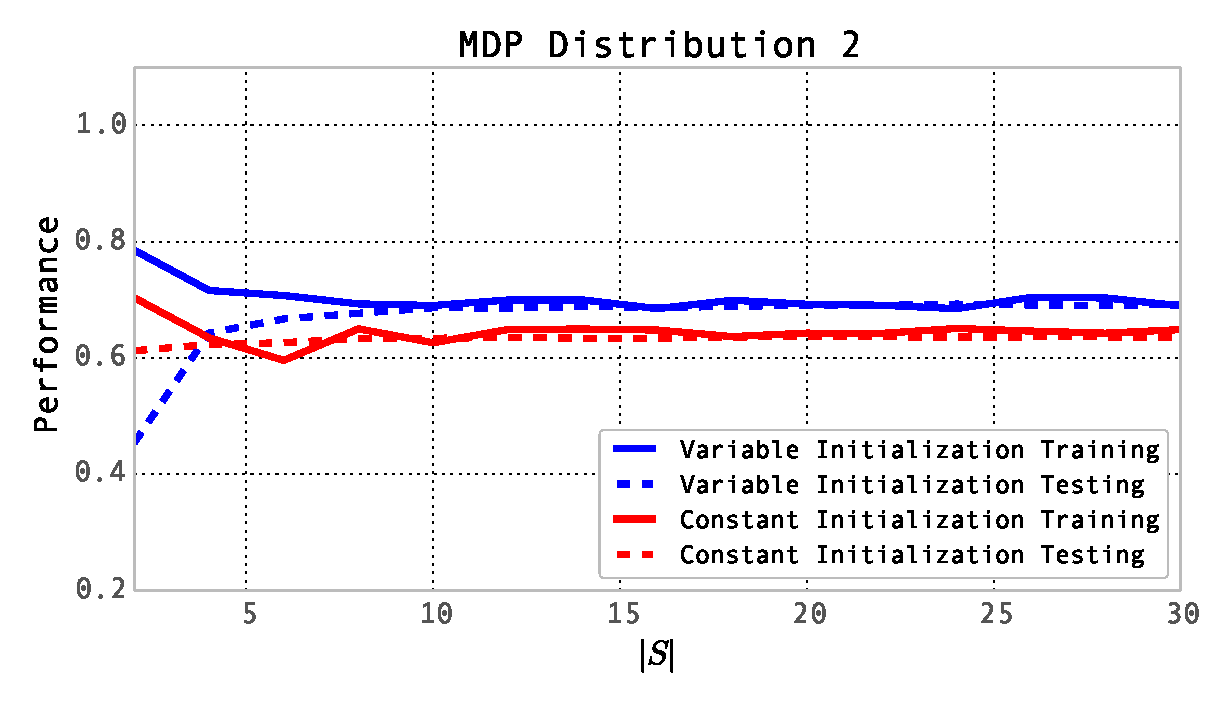
\includegraphics[width=.45\columnwidth]{images/mdp_distribution2}
\end{tabular}
\caption{Training and testing performance for two distributions in the 5-state chain environment. Performance is measured as the probability of converging to the optimal policy.}
\label{fig:underfit}
\end{figure*}

Since performance on the training set of MDP samples can be deceptive, we would like a way to bound the {\em generalization error}. The generalization error is the difference in the performance of a selected algorithm on a training set and its performance on the full distribution. More formally, let $\mathcal{A}$ be the space of parameterized algorithms and let $\mathcal{F}$ be the space of evaluation functions of each algorithm $a \in \mathcal{A}$ such that for all $f_a \in \mathcal{F}$, $f_a : \mathcal{D} \rightarrow [0,1]$, where $\mathcal{D}$ is the space of MDPs our MDP distribution spans. Let $S$ be a sample $z_1,\dots, z_m$, chosen from a distribution $D$ on $\mathcal{D}$. Then the generalization error of algorithm $a$ is $| \hat{E}_S[f_a] - E[f_a] |$, where $\hat{E}_S[f_a]= \frac{1}{m}\sum_{i=1}^m f_a(z_i)$ is the expected performance of $a$ on the training data, and $E[f_a]= \int_\mathcal{D} f_a(z) D(z) dz$ is the expected performance of $a$ on the full distribution.





%\section{Conclusion}

\bibliographystyle{plain}
\bibliography{groundhog}